\chapter{Analýza podobných webových služeb}
\label{analyza}

V~současné době neexistuje žádná webová služba stejného typu, proto budou v~této diplomové práci zanalyzovány webové služby, které zpracovávají některou žádanou funkcionalitu. Konkrétně se jedná o~tyto webové služby:
\begin{itemize}
	\item \textbf{BlaBlaCar.cz} \cite{blablacar} (\url{https://www.blablacar.cz}) -- Velmi podobná problematika, jen v~jiném kabátu. Obsahuje vyhledávání nabídek a hodnocení uživatelů, kteří zadávají své jízdy ke spolujízdě, případně se k~těmto spolujízdám přihlašují.
	\item \textbf{Couchsurfing.com} \cite{couchsurfing} (\url{https://www.couchsurfing.com}) -- Komunita lidí, kteří rádi cestují a chtějí poznávat svět, ale nechtějí platit velké množství peněz za hotely. Pro tuto práci jsou důležitými prvky hodnocení uživatelů, jejich ověření a lokalizované vyhledávání nabídek.
	\item \textbf{Sreality.cz} \cite{sreality} (\url{https://www.sreality.cz}) -- Realitní agentura, která je pro tuto práci zajímavá čistým a přehledným vzhledem svojí webové aplikace a také rychlým vyhledáváním nabídek přímo v~mapě.
	\item \textbf{Aukro.cz} \cite{aukro} (\url{http://aukro.cz}) -- Prodej výrobků, který zaujme zpracováním hodnocení uživatelů (prodejců).
	\item \textbf{Zonky.cz} \cite{zonky} (\url{https://zonky.cz}) -- Bankovní a nebankovní půjčky. S~prací mají společnou přímou pomoc mezi lidmi, a tím pádem možnost výhodnějších nabídek.
\end{itemize}

\newpage
\section{BlaBlaCar}
\label{analyza:blablacar}

BlaBlaCar je přední světová komunita spolujízdy, která spojuje řidiče a cestující na stejné trase, a umožňuje tak levné meziměstské cestování \cite{blablacar}.

Na základě tohoto jednoduchého principu si lidé mohou přisednout k~někomu jako spolucestující. Tímto způsobem se tak dostanou k~častokrát levnější a pohodlnější formě přepravy. Pro řidiče je výhodou částečné proplacení jízdy (pohonných hmot) těmito spolucestujícími.

Níže jsou uvedeny všechny důležité stránky webu BlaBlaCar a u~každé takové stránky je definován seznam pozitivních a negativních vlastností.

\subsection{Hlavní stránka}
Viz obrázek \ref{fig:blablacar:homepage}.
\begin{figure}[h]
    \centering
    
\includegraphics[width=1.0\textwidth]{media/blablacar/homepage.png}
    \caption{BlaBlaCar.cz -- Hlavní stránka}
    \label{fig:blablacar:homepage}
\end{figure}
\subsubsection*{Pozitiva}
\begin{itemize}
    \item[+] \textbf{Přehlednost} -- Na stránce jsou výrazně viditelné dva nejdůležitější typy úkonů a to \textit{Nabídnutí jízdy} a \textit{Vyhledávání jízdy}. I~v~této práci bude brán ohled na to, aby každá důležitá akce měla vysokou prioritu.
    \item[+] \textbf{Ostatní možnosti} -- V~pravém horním rohu je dostupný profil uživatele a nová upozornění na události týkající se uživatelského profilu.
    \item[+] \textbf{Jak to funguje} -- Každému uživateli na první pohled nemusí být jasné, o~co se přesně jedná. Proto web BlaBlaCar.cz na své úvodní stránce uvádí postup jak se na spolujízdu registrovat.
    \item[+] \textbf{Oblíbené trasy} -- Seznam tří nejoblíbenějších tras uživatelů.
\end{itemize}
\subsubsection*{Negativa}
\begin{itemize}
    \item[-] \textbf{Žádná negativa na této stránce nejsou pozorována.}
\end{itemize}


%%%%%%%%%%%%%%%%%%%%%%%%%%%%%%%%%%%%%%%%%%%%%%%%%%%%%%%%%%%%%%%%%%%%%%%%%%%%%%%%%%%%%%%%%%%%%%%%%%%%%%%%%%%%%%%%%%%%%%%%

\newpage
\subsection{Vyhledávání jízdy}
Viz obrázek \ref{fig:blablacar:search}.
\begin{figure}[h]
    \centering
    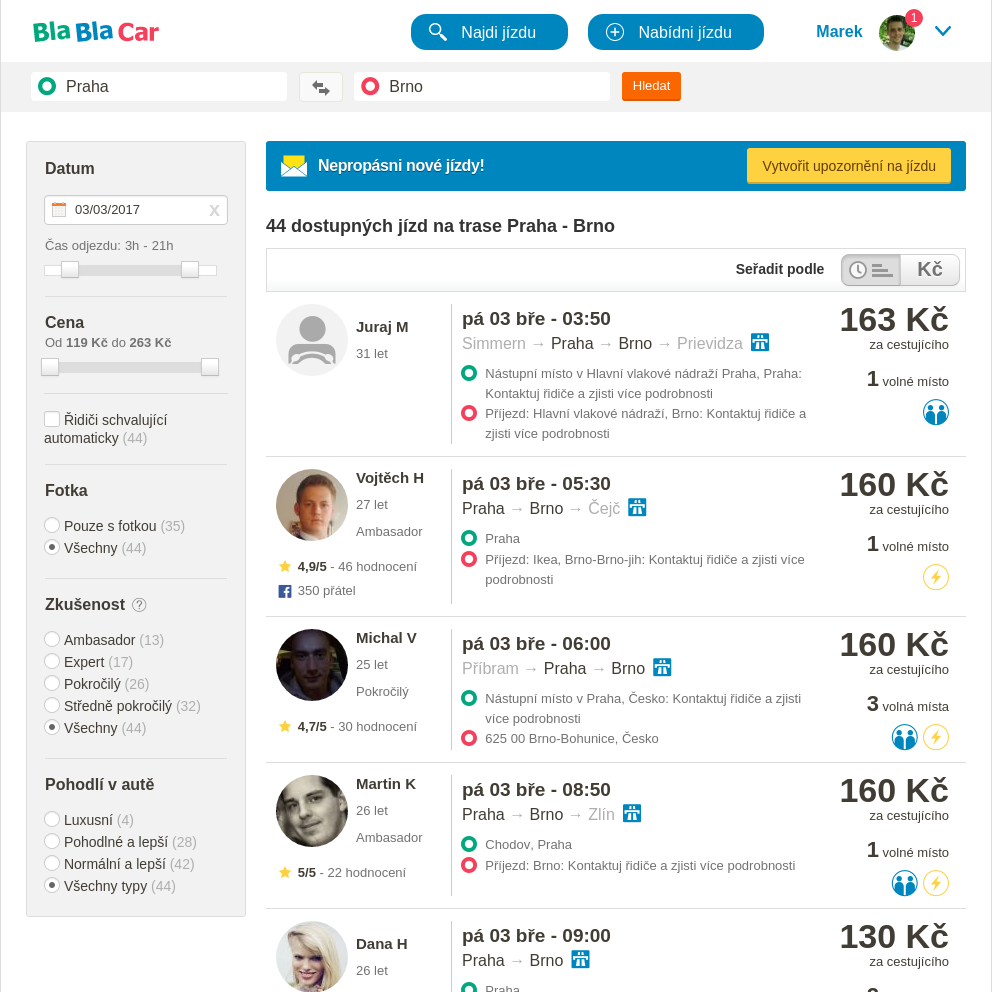
\includegraphics[width=1.0\textwidth]{media/blablacar/search.png}
    \caption{BlaBlaCar.cz -- Vyhledávání nabídek}
    \label{fig:blablacar:search}
\end{figure}
\subsubsection*{Pozitiva}
\begin{itemize}
    \item[+] \textbf{Informativnost} -- Hned na první pohled uživatel vidí všechny relevantní informace: čas, cenu, počet volných míst, délku trasy a hodnocení daného řidiče.
    \item[+] \textbf{Filtry} -- Možnost filtrovaní požadavků na základě zkušeností řidiče a pohodlí auta považuji za nejdůležitější.
    \item[+] \textbf{Možnost řazení} -- Seřazení nabídek podle ceny a času odjezdu je určitě velmi vítaná a potřebná vlastnost.
\end{itemize}
\subsubsection*{Negativa}
\begin{itemize}
    \item[-] \textbf{Nedostupnost profilu řidiče na jeden klik} -- Na první pohled očekávaná funkcionalita (existence předělu mezi cestou a profilem řidiče), při které by se uživatel po kliknutí myší na pravou část nabídky dostal na bližší informace o~jízdě a po kliknutí na levou část nabídky dostal na profil řidiče. Tohoto problému se při návrhu uživatelského rozhraní budu snažit vyvarovat.
\end{itemize}


%%%%%%%%%%%%%%%%%%%%%%%%%%%%%%%%%%%%%%%%%%%%%%%%%%%%%%%%%%%%%%%%%%%%%%%%%%%%%%%%%%%%%%%%%%%%%%%%%%%%%%%%%%%%%%%%%%%%%%%%

\newpage
\subsection{Detail jízdy}
Viz obrázek \ref{fig:blablacar:detail}.
\begin{figure}[h]
    \centering
    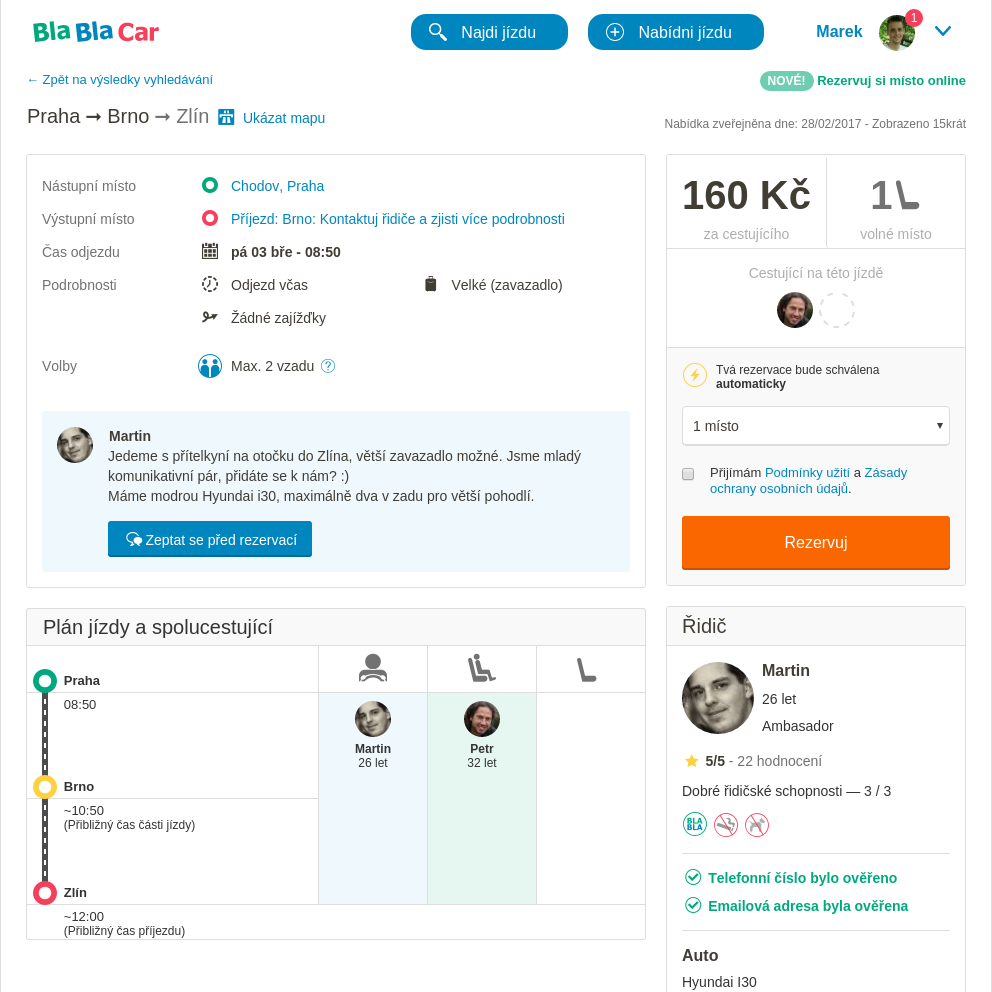
\includegraphics[width=1.0\textwidth]{media/blablacar/detail.png}
    \caption{BlaBlaCar.cz -- Detail jízdy}
    \label{fig:blablacar:detail}
\end{figure}
\subsubsection*{Pozitiva}
\begin{itemize}
    \item[+] \textbf{Harmonogram} -- Graficky velmi pěkně řešený přehled celé jízdy a spolucestujících včetně časů odjezdů a příjezdů.
    \item[+] \textbf{Spolucestující} -- Možnost vidět kdo s~vámi cestuje je vítaná, jelikož s~někým se rádi svezete a někomu se naopak raději vyhnete.
    \item[+] \textbf{Podrobnosti} -- Tímto se řidič vyhne nepříjemnostem s~velkým počtem zavazadel a uživatel s~delšími zajížďkami řidiče.
\end{itemize}
\subsubsection*{Negativa}
\begin{itemize}
    \item[-] \textbf{Žádná negativa na této stránce nejsou pozorována.}
\end{itemize}


%%%%%%%%%%%%%%%%%%%%%%%%%%%%%%%%%%%%%%%%%%%%%%%%%%%%%%%%%%%%%%%%%%%%%%%%%%%%%%%%%%%%%%%%%%%%%%%%%%%%%%%%%%%%%%%%%%%%%%%%

\newpage
\subsection{Nabídnutí jízdy}
Viz obrázky \ref{fig:blablacar:offer} a \ref{fig:blablacar:offer2}.
\begin{figure}[h]
    \centering
    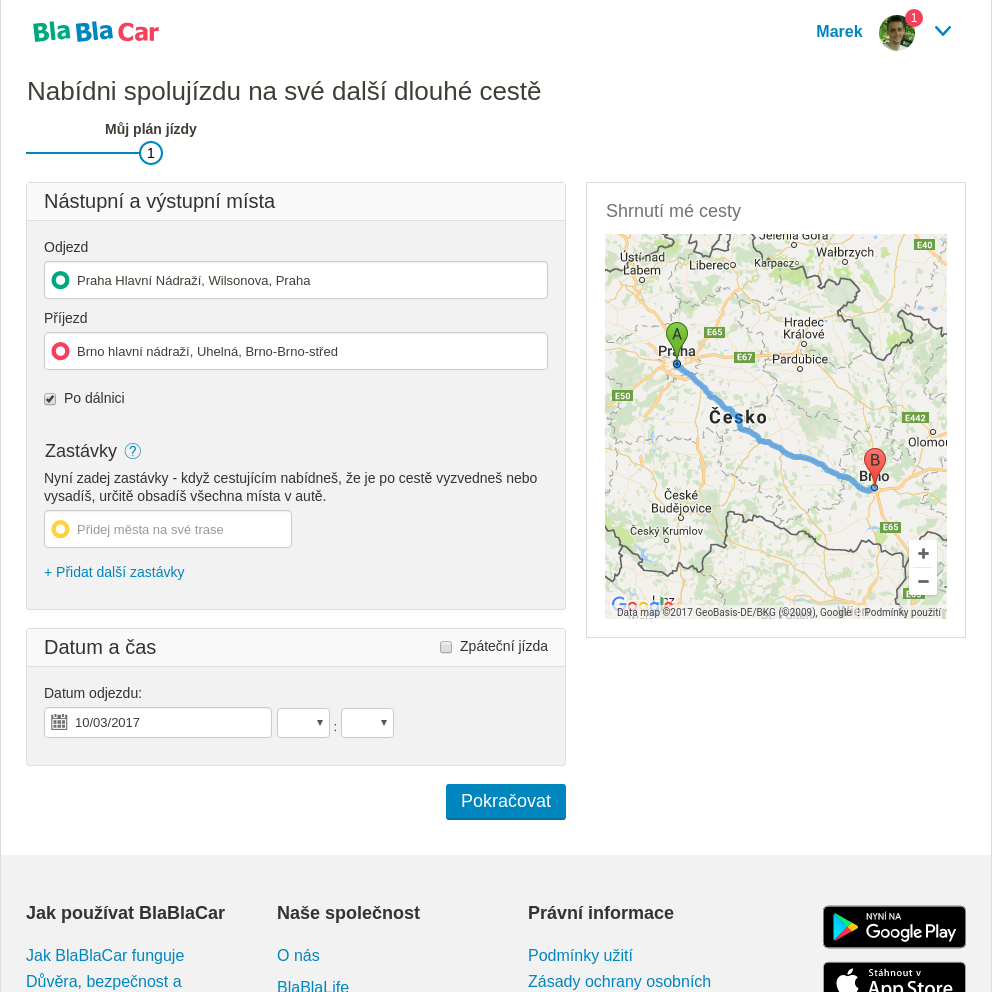
\includegraphics[width=1.0\textwidth]{media/blablacar/offer.png}
    \caption{BlaBlaCar.cz -- Zadání nové jízdy -- Harmonogram}
    \label{fig:blablacar:offer}
\end{figure}
\begin{figure}[h]
    \centering
    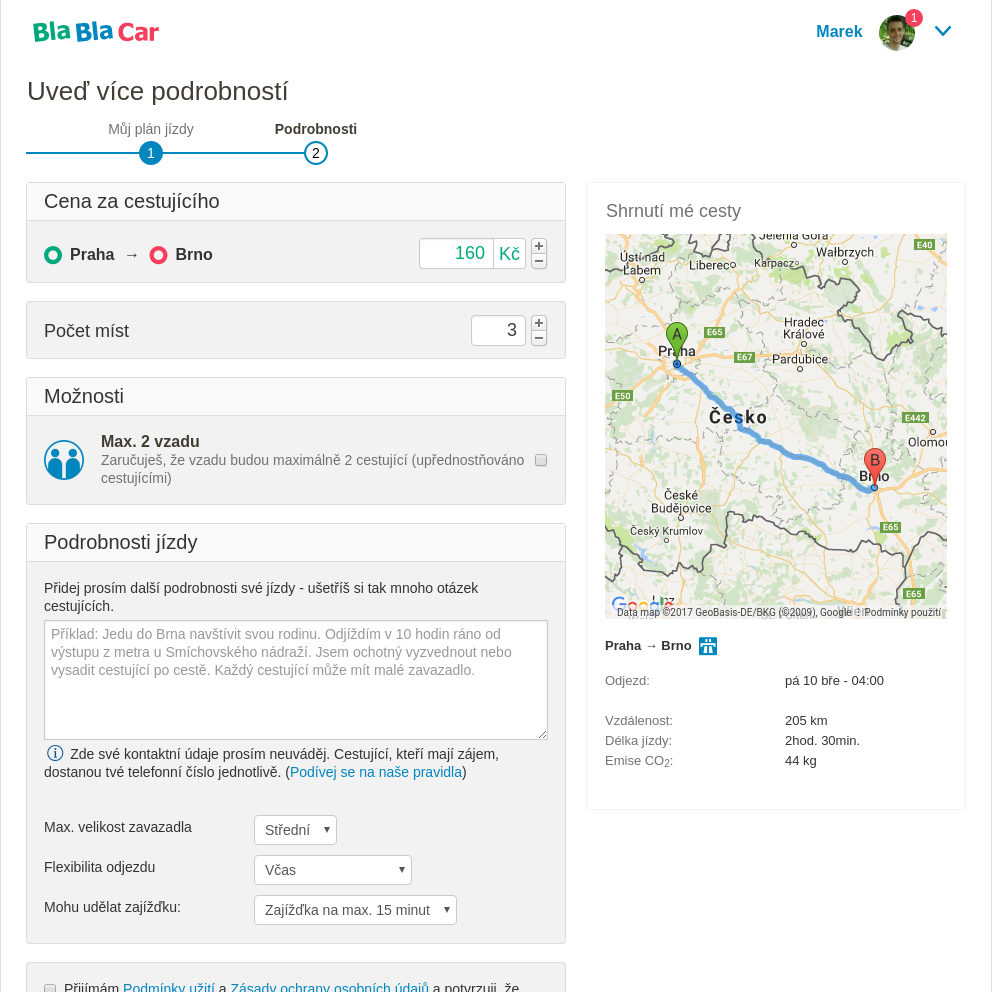
\includegraphics[width=1.0\textwidth]{media/blablacar/offer2.png}
    \caption{BlaBlaCar.cz -- Zadání nové jízdy -- Podrobnosti}
    \label{fig:blablacar:offer2}
\end{figure}
\subsubsection*{Pozitiva}
\begin{itemize}
    \item[+] \textbf{Krok za krokem} -- Uživatel postupně prochází všemi důležitými aspekty nabídky jízdy.
    \item[+] \textbf{Přijatelné UI} -- Všechno je na svém místě a výrazně odlišené od ostatních položek.
    \item[+] \textbf{Doporučená cena} -- Automatické vyplnění ceny na základě ostatních nabídek a vzdálenosti.
    \item[+] \textbf{Mapa} -- Mapa s~celkovým shrnutím vzdálenosti a trvání jízdy.
\end{itemize}
\subsubsection*{Negativa}
\begin{itemize}
    \item[-] \textbf{Žádná negativa na této stránce nejsou pozorována.}
\end{itemize}


%%%%%%%%%%%%%%%%%%%%%%%%%%%%%%%%%%%%%%%%%%%%%%%%%%%%%%%%%%%%%%%%%%%%%%%%%%%%%%%%%%%%%%%%%%%%%%%%%%%%%%%%%%%%%%%%%%%%%%%%

\newpage
\subsection{Profil uživatele}
Viz obrázek \ref{fig:blablacar:profile}.
\begin{figure}[h]
    \centering
    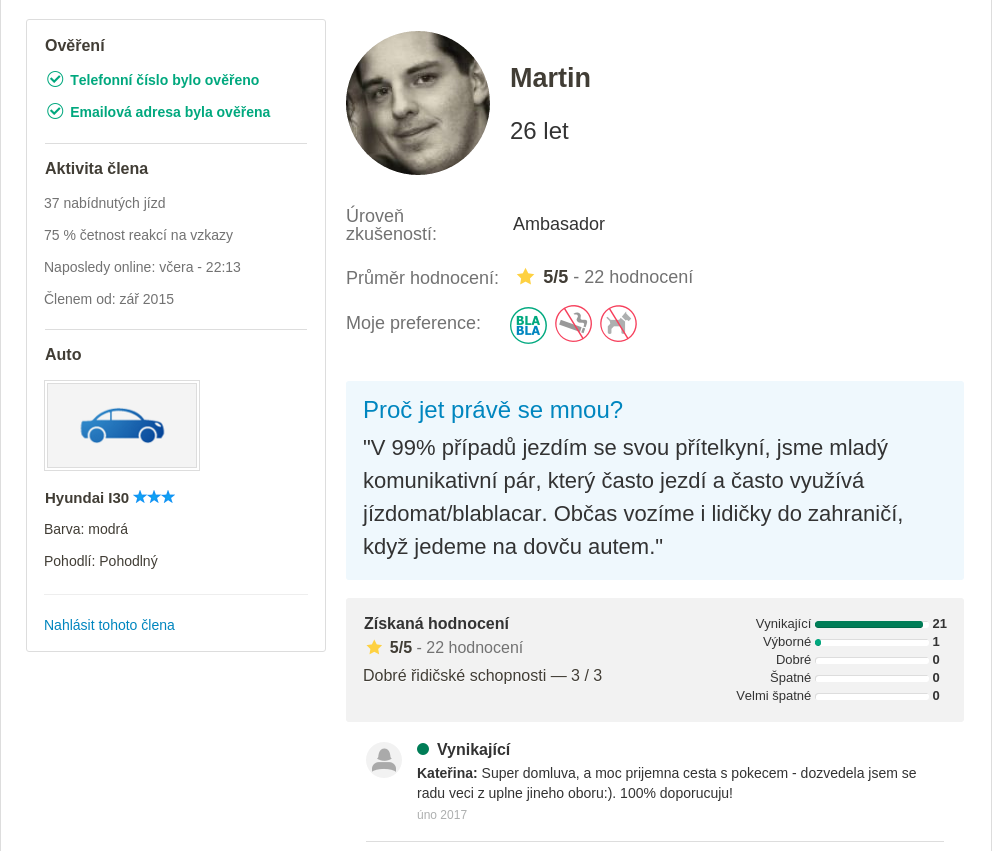
\includegraphics[width=1.0\textwidth]{media/blablacar/profile.png}
    \caption{BlaBlaCar.cz -- Profil uživatele}
    \label{fig:blablacar:profile}
\end{figure}
\subsubsection*{Pozitiva}
\begin{itemize}
    \item[+] \textbf{Informativnost} -- Recenze, typ auta, počet nabídnutých jízd. Uživatel se jednoduše dozví vše, co potřebuje bez nutnosti přecházet na další stránku.
    \item[+] \textbf{Ověření} -- Různé úrovně ověření každého uživatele.
\end{itemize}
\subsubsection*{Negativa}
\begin{itemize}
    \item[-] \textbf{Žádná negativa na této stránce nejsou pozorována.}
\end{itemize}


%%%%%%%%%%%%%%%%%%%%%%%%%%%%%%%%%%%%%%%%%%%%%%%%%%%%%%%%%%%%%%%%%%%%%%%%%%%%%%%%%%%%%%%%%%%%%%%%%%%%%%%%%%%%%%%%%%%%%%%%

\newpage
\subsection{Shrnutí}
Pro účel aplikace jsou nejdůležitější dvě stránky, které BlaBlaCar poskytuje a to \textit{Vyhledávání jízdy} a \textit{Detail jízdy}.

Při návrhu uživatelského rozhraní bude brán zřetel na poskytnutí možnosti filtrování a také seřazení nabídek. Důležité bude zakomponovat rozdílnost kliknutí na uživatele, která uživatele dostane na jeho profil, resp. samotné nabídky, která uživatele přesměruje na bližší informace o~dané nabídce.

I~napříč tomu, že v~aplikaci neexistují spolucestující, tak si beru příklad z~této vlastnosti BlaBlaCar a v~detailu nabídky zvážím výpis historie s~daným uživatelem, která slouží velmi podobnému účelu.

Hodnocení uživatelů je řešeno pomocí až pěti hvězdiček.
\newpage
\section{Couchsurfing}
\label{analyza:couchsurfing}

Ubytování bývá drahé a proto existují lidé, kteří na pár nocí vypůjčují svůj gauč a tím pomohou někomu poznat jejich město a zemi. Pro cestující z~toho plyne ještě jeden pozitivní dopad -- skvělé informace, které by se nikde jinde nedozvěděli, a to přímo od místního člověka.

Pravě touto problematikou se zabývá webová služba Couchsurfing \cite{couchsurfing}.
\subsection{Hlavní stránka}
Viz obrázek \ref{fig:couchsurfing:homepage}.
\begin{figure}[h]
    \centering
    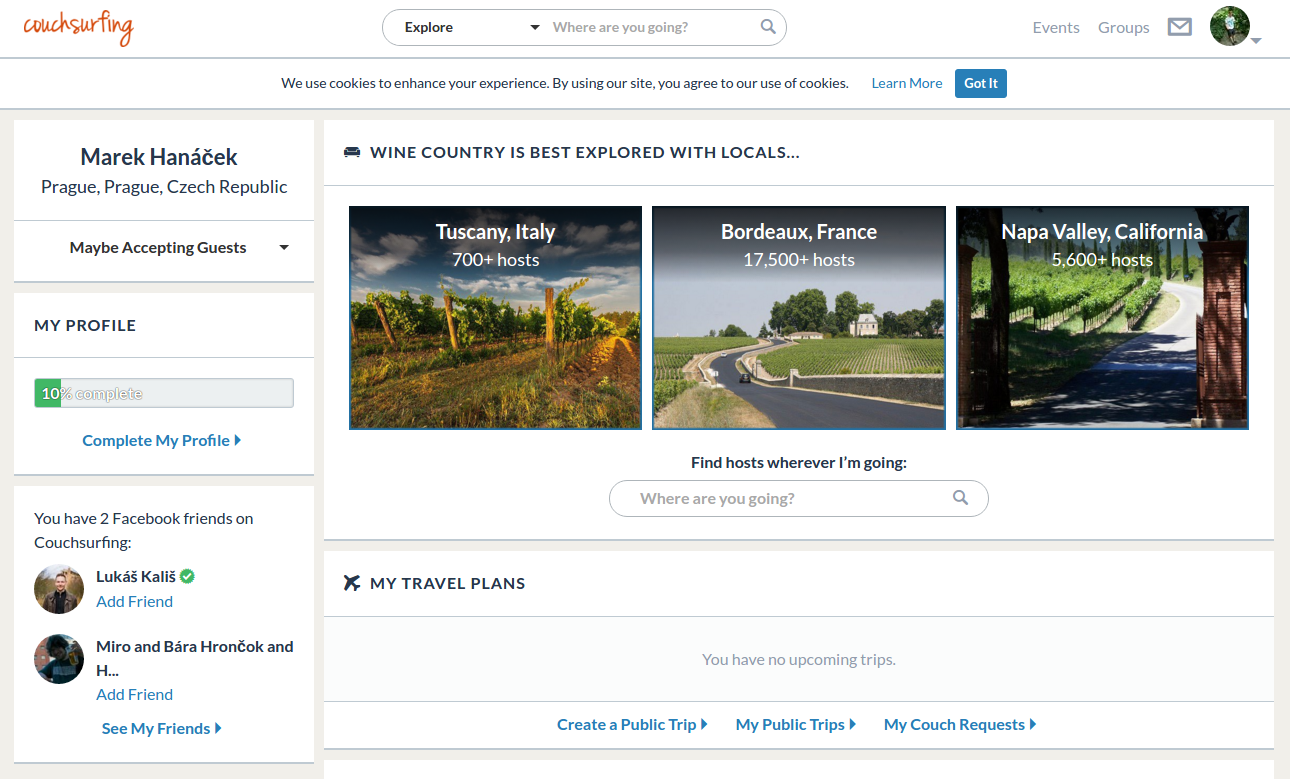
\includegraphics[width=1.0\textwidth]{media/couchsurfing/homepage.png}
    \caption{Couchsurfing.com -- Hlavní stránka}
    \label{fig:couchsurfing:homepage}
\end{figure}
\subsubsection*{Pozitiva}
\begin{itemize}
    \item[+] \textbf{Přehlednost} -- Všechno důležité na jednom místě a přehledně oddělené.
    \item[+] \textbf{Vyhledávací okno} -- Rychlé vyhledávací okno v~horní části stránky.
\end{itemize}
\subsubsection*{Negativa}
\begin{itemize}
    \item[-] \textbf{Stránka je dlouhá} -- Pro zobrazení veškerého obsahu je potřeba se dlouze posouvat po stránce.
\end{itemize}


%%%%%%%%%%%%%%%%%%%%%%%%%%%%%%%%%%%%%%%%%%%%%%%%%%%%%%%%%%%%%%%%%%%%%%%%%%%%%%%%%%%%%%%%%%%%%%%%%%%%%%%%%%%%%%%%%%%%%%%%

\newpage
\subsection{Vyhledávání ubytovaní}
Viz obrázek \ref{fig:couchsurfing:search}.
\begin{figure}[h]
    \centering
    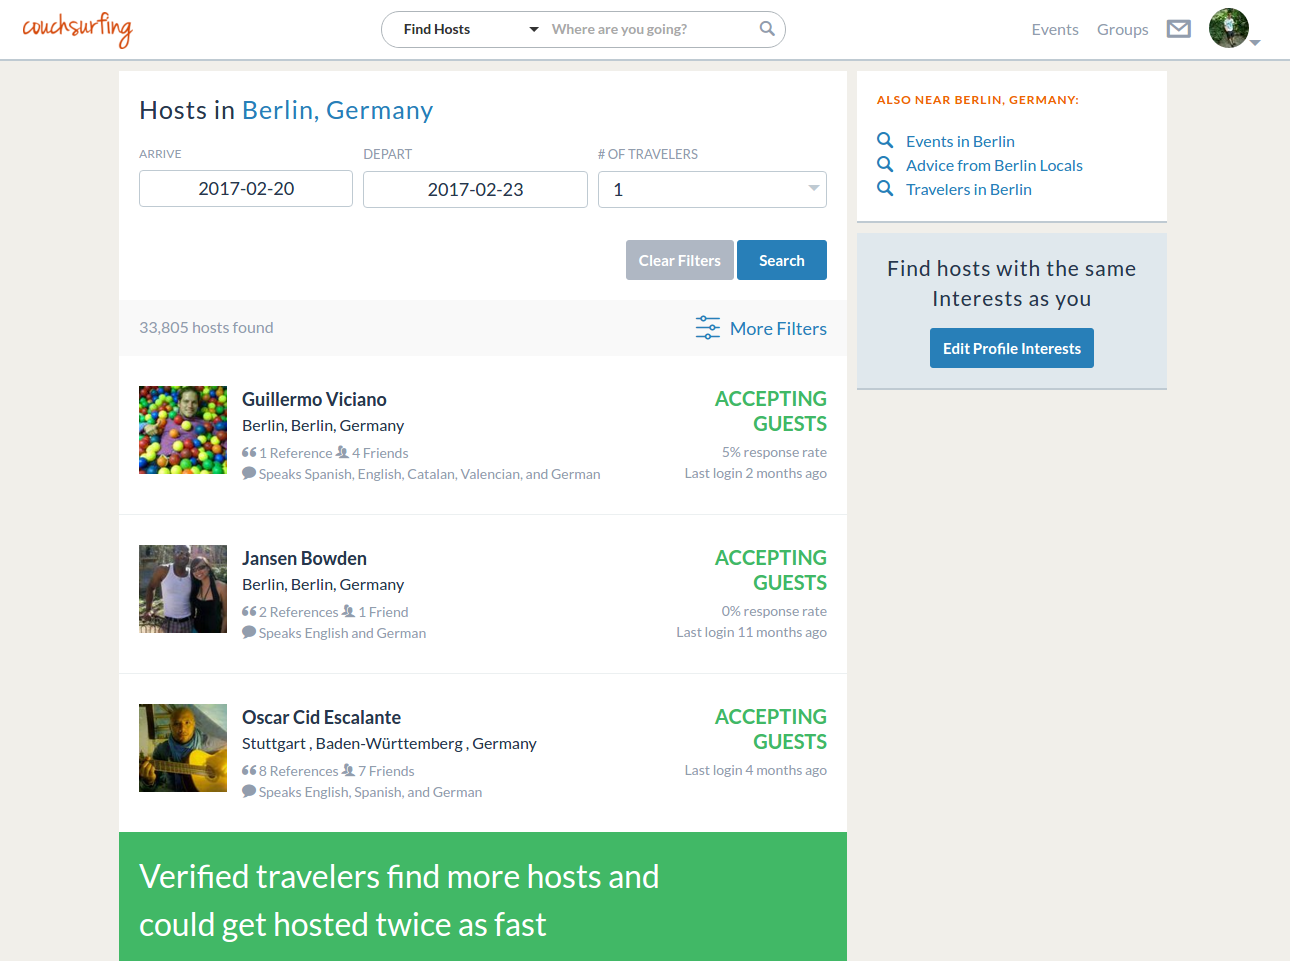
\includegraphics[width=1.0\textwidth]{media/couchsurfing/search.png}
    \caption{Couchsurfing.com -- Vyhledávání ubytování}
    \label{fig:couchsurfing:search}
\end{figure}
\subsubsection*{Pozitiva}
\begin{itemize}
    \item[+] \textbf{Jednoduchost}
    \item[+] \textbf{Filtry} -- Všechno důležité s~možností rozšířeného filtru.
    \item[+] \textbf{Status} -- Ověření uživatelé jsou jasně viditelní.
\end{itemize}
\subsubsection*{Negativa}
\begin{itemize}
    \item[-] \textbf{Žádná negativa na této stránce nejsou pozorována.}
\end{itemize}


%%%%%%%%%%%%%%%%%%%%%%%%%%%%%%%%%%%%%%%%%%%%%%%%%%%%%%%%%%%%%%%%%%%%%%%%%%%%%%%%%%%%%%%%%%%%%%%%%%%%%%%%%%%%%%%%%%%%%%%%

\newpage
\subsection{Profil uživatele}
Viz obrázek \ref{fig:couchsurfing:profile}.
\begin{figure}[h]
    \centering
    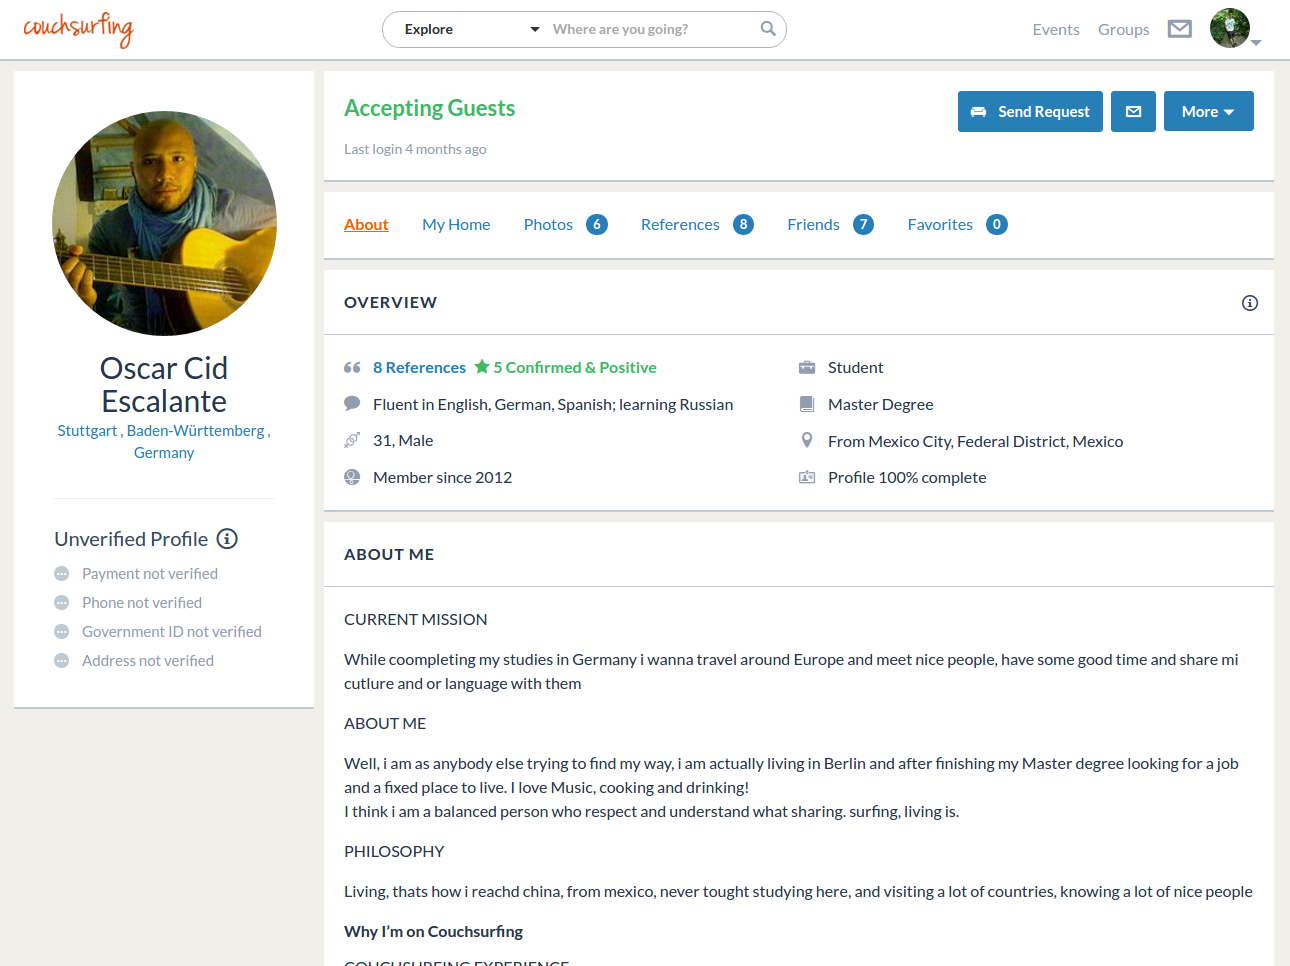
\includegraphics[width=1.0\textwidth]{media/couchsurfing/profile.png}
    \caption{Couchsurfing.com -- Profil uživatele}
    \label{fig:couchsurfing:profile}
\end{figure}
\subsubsection*{Pozitiva}
\begin{itemize}
    \item[+] \textbf{Informativnost} -- Všechno kompaktně na jednom místě a přehledně.
    \item[+] \textbf{O~uživateli} -- Popis uživatele uživatelem samotným. Jistě vítaná funkcionalita.
\end{itemize}
\subsubsection*{Negativa}
\begin{itemize}
    \item[-] \textbf{Žádná negativa na této stránce nejsou pozorována.}
\end{itemize}


%%%%%%%%%%%%%%%%%%%%%%%%%%%%%%%%%%%%%%%%%%%%%%%%%%%%%%%%%%%%%%%%%%%%%%%%%%%%%%%%%%%%%%%%%%%%%%%%%%%%%%%%%%%%%%%%%%%%%%%%

\newpage
\subsection{Shrnutí}
Celkově se webová aplikace Couchsurfing jeví velmi dobře řešená.

Důležitým mottem, se kterým je budována webová aplikace, je být \textbf{přehledný}. Každá podstránka by měla obsahovat vše co je potřeba a nic víc. Zajímavou myšlenkou je existence \textbf{verifikovaných uživatelů}, která by v~této práci vytvořila důvěru a určitou záruku korektního jednání při výměně peněz. Nevýhodu je velmi dlouhé provedení úvodní stránky, čehož je potřeba se vyvarovat a tím pádem ulehčit uživateli orientaci na stránce.
\newpage
\section{SReality.cz}
\label{analyza:sreality}
Realitní agentura SReality si vytvořila webovou aplikaci, která má ulehčovat uživatelům výběr domu či bytu, ve kterém stráví následující roky svého života. Takové rozhodnutí bývá velmi náročné a proto od Sreality.cz očekávám jasné podání informací a hlavně přijatelné uživatelské prostředí. Toto očekávání je znásobené ještě tím, že uživatelé, kteří navštíví danou stránku, mohou být z různých věkových skupin.\\

\subsection{Home page}
\begin{figure}[h]
    \centering
    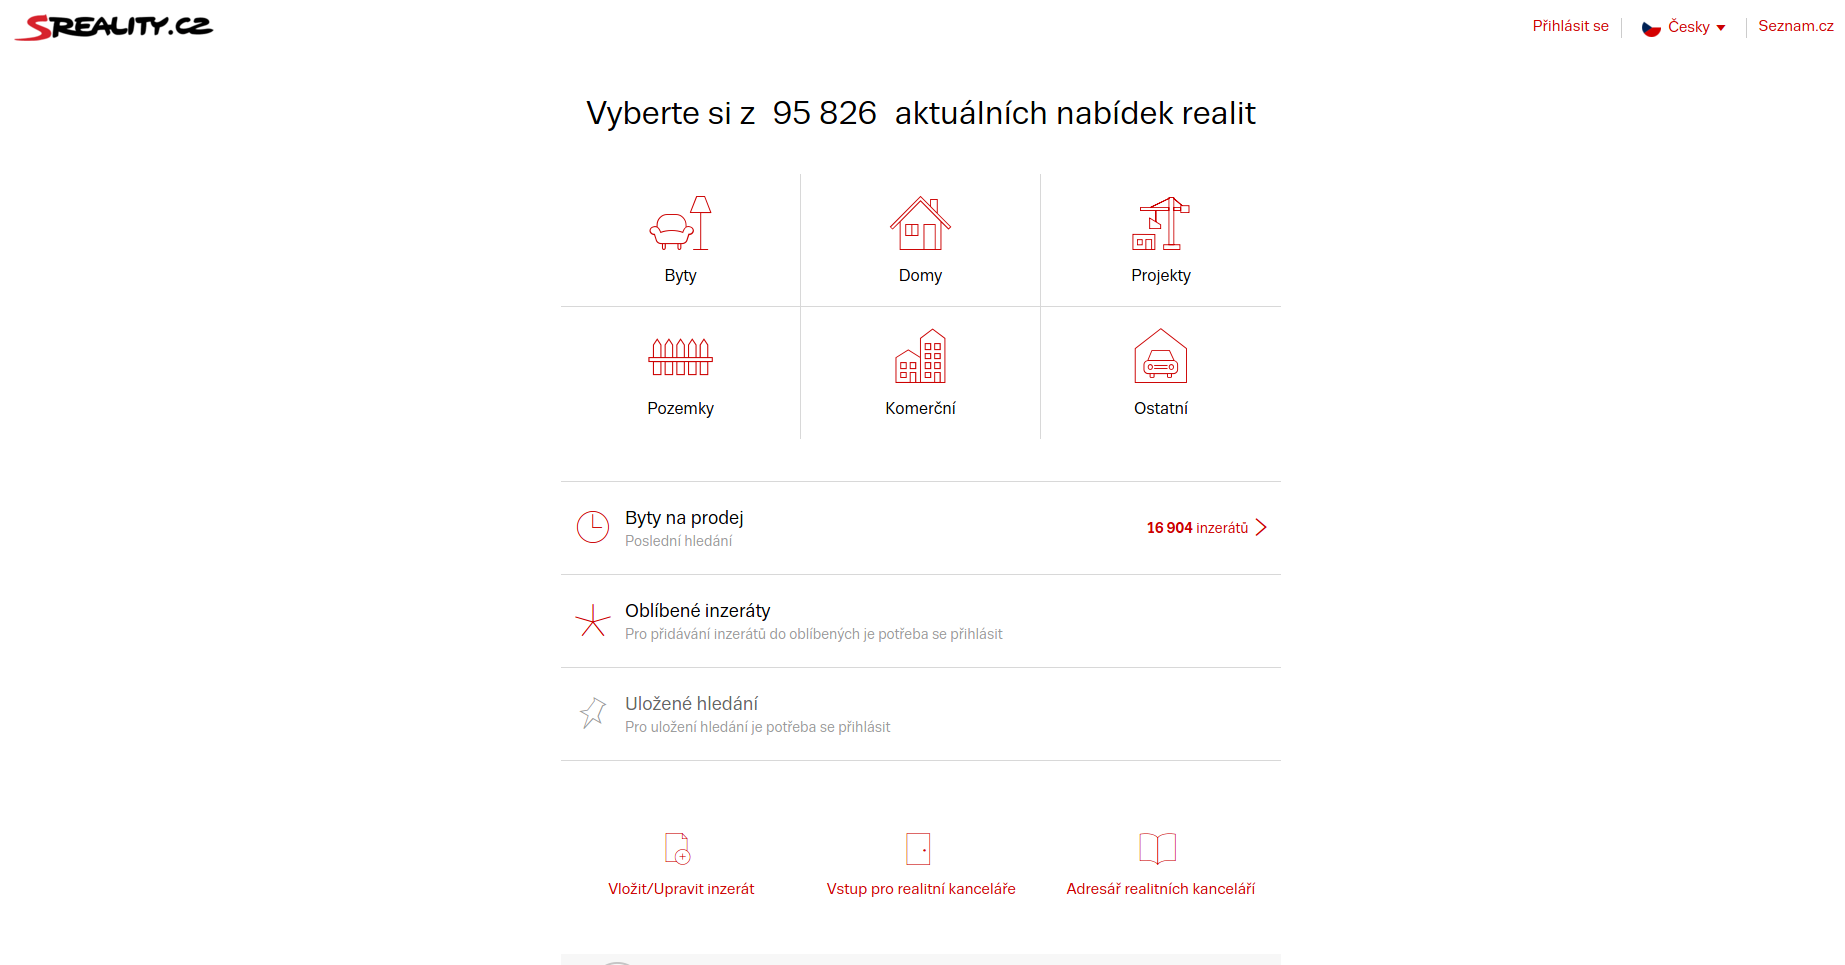
\includegraphics[width=1.0\textwidth]{media/sreality/homepage.png}
    \caption{Hlavní stránka webu Sreality.cz}
    \label{fig:sreality:homepage}
\end{figure}
\subsubsection*{Pozitiva}
\begin{itemize}
    \item[+] \textbf{Jednoduchost} -- Bílé prostředí, které obsahuje pouze černé nápisy a červené obrysové nákresy. Velmi jednoduché a přehledné řešení.
    \item[+] \textbf{Poslední a oblíbené vyhledávání} -- Speciální možnosti, které ulehčí hledání uživatelům, kteří již na dané stránce byli a možná si už i nějaké nabídky vybrali.
\end{itemize}
\subsubsection*{Negativa}
\begin{itemize}
    \item[-] \textbf{Nevidím}
\end{itemize}


%%%%%%%%%%%%%%%%%%%%%%%%%%%%%%%%%%%%%%%%%%%%%%%%%%%%%%%%%%%%%%%%%%%%%%%%%%%%%%%%%%%%%%%%%%%%%%%%%%%%%%%%%%%%%%%%%%%%%%%%

\newpage
\subsection{Vyhledávání realit}
\begin{figure}[h]
    \centering
    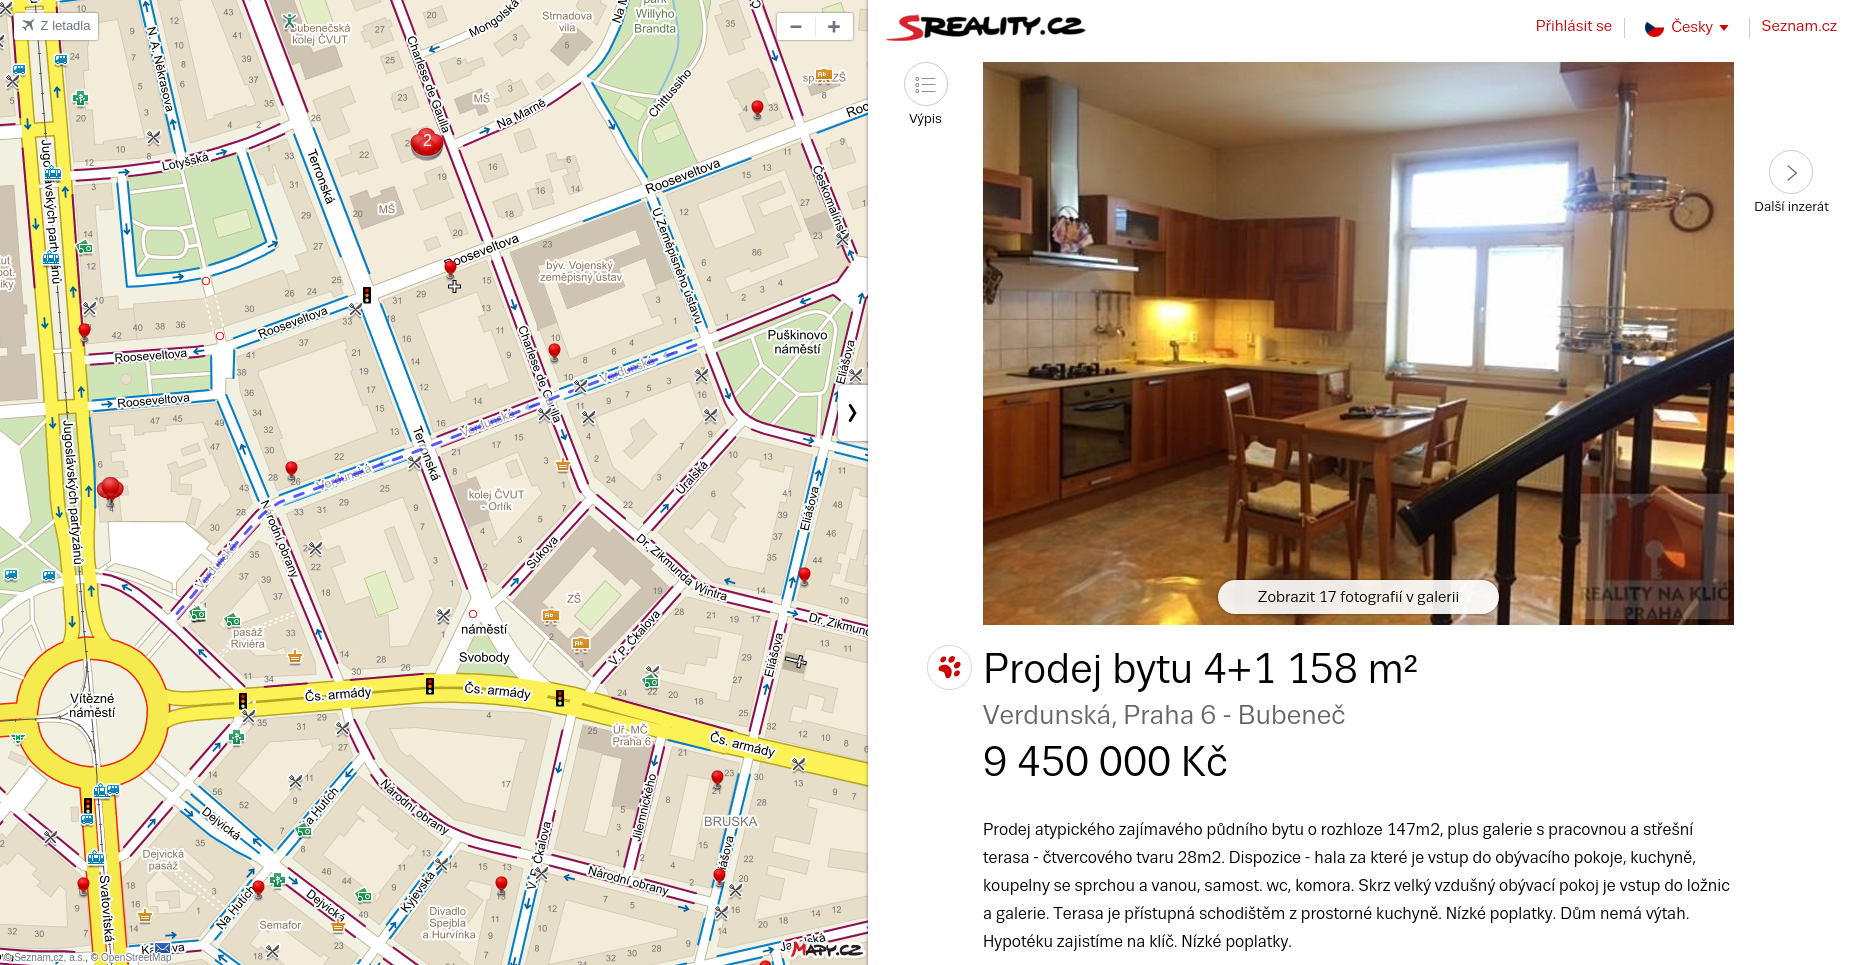
\includegraphics[width=1.0\textwidth]{media/sreality/detail.png}
    \caption{Detail nabídky na webu Sreality.cz}
    \label{fig:sreality:detail}
\end{figure}
\begin{figure}[h]
    \centering
    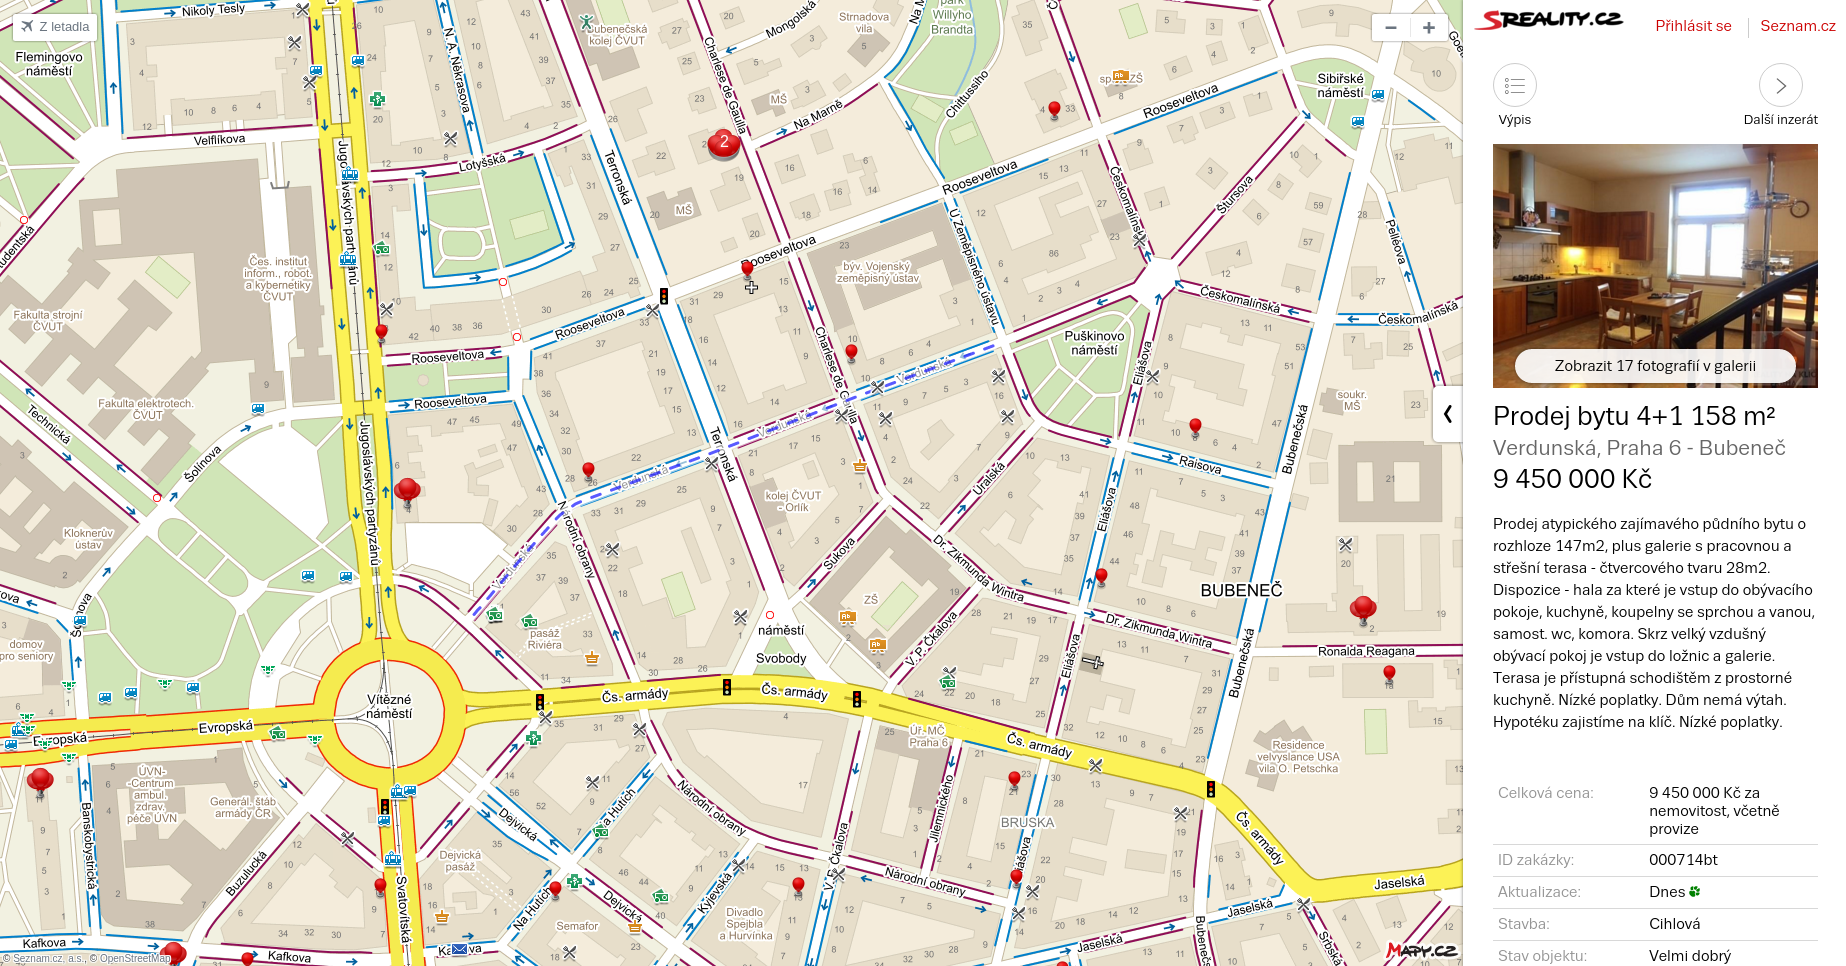
\includegraphics[width=1.0\textwidth]{media/sreality/detail-big-map.png}
    \caption{Detail nabídky na webu Sreality.cz - větší mapa}
    \label{fig:sreality:detail-big-map}
\end{figure}
\subsubsection*{Pozitiva}
\begin{itemize}
    \item[+] \textbf{Mapa} -- Krásné propojení map od společnosti Seznam.cz a vyhledávání. Navíc je hned vidět jak daleko se nachází zastávka městské hromadné dopravy nebo nejbližší supermarket a další.
    \item[+] \textbf{Lišta s náhledem nabídky} -- Informativní popis všech vlastností dané nabídky.
    \item[+] \textbf{Zvětšení/zmenšení} -- Uživatel má možnost zvětšit, nebo zmenšit mapu a tím pádem vidět méně či naopak více z obsahu.
\end{itemize}
\subsubsection*{Negativa}
\begin{itemize}
    \item[-] \textbf{Nemožnost čistého náhledu bez mapy} -- Při užším a delším vybírání je možné, že lokalitu mám jako uživatel dobře zmapovanou a tím pádem nepotřebuji vidět mapu (ani v malé formě) na levé straně obrazovky.
\end{itemize}


%%%%%%%%%%%%%%%%%%%%%%%%%%%%%%%%%%%%%%%%%%%%%%%%%%%%%%%%%%%%%%%%%%%%%%%%%%%%%%%%%%%%%%%%%%%%%%%%%%%%%%%%%%%%%%%%%%%%%%%%

\newpage
\subsection{Shrnutí}
Celkově se mi webová aplikace Sreality.cz jeví jako velmi dobře řešená.

Nejzajímavějším aspektem Sreality.cz se mi jeví přítomnost \textbf{mapy}, která ulehčuje a urychluje výběr. Tuto vlastnost určitě chci zakomponovat do své webové aplikace. Forma přepínání mezi mapou a obsahem je řešená \textbf{jednoduše} a uživatelsky přijatelně. Podle mě je však dobré se \textbf{vyvarovat nutnosti vždy zobrazovat mapu} a ponechat tuto funkcionalitu jen jako možnost.

Hodnocení uživatelů zde není nijak řešené.
\newpage
\section{Aukro}

\label{analyza:aukro}

Webová aplikace, která se nezabývá jen aukcemi, ale také normálním prodejem zboží. Protože je to ve své podstatě e-shop, tak od něj očekávám dobře zvolené kategorie, detaily v popise zboží a v případě Aukra i výrazné zobrazení hodnocení prodejců zboží.

\subsection{Home page}
\begin{figure}[h]
    \centering
    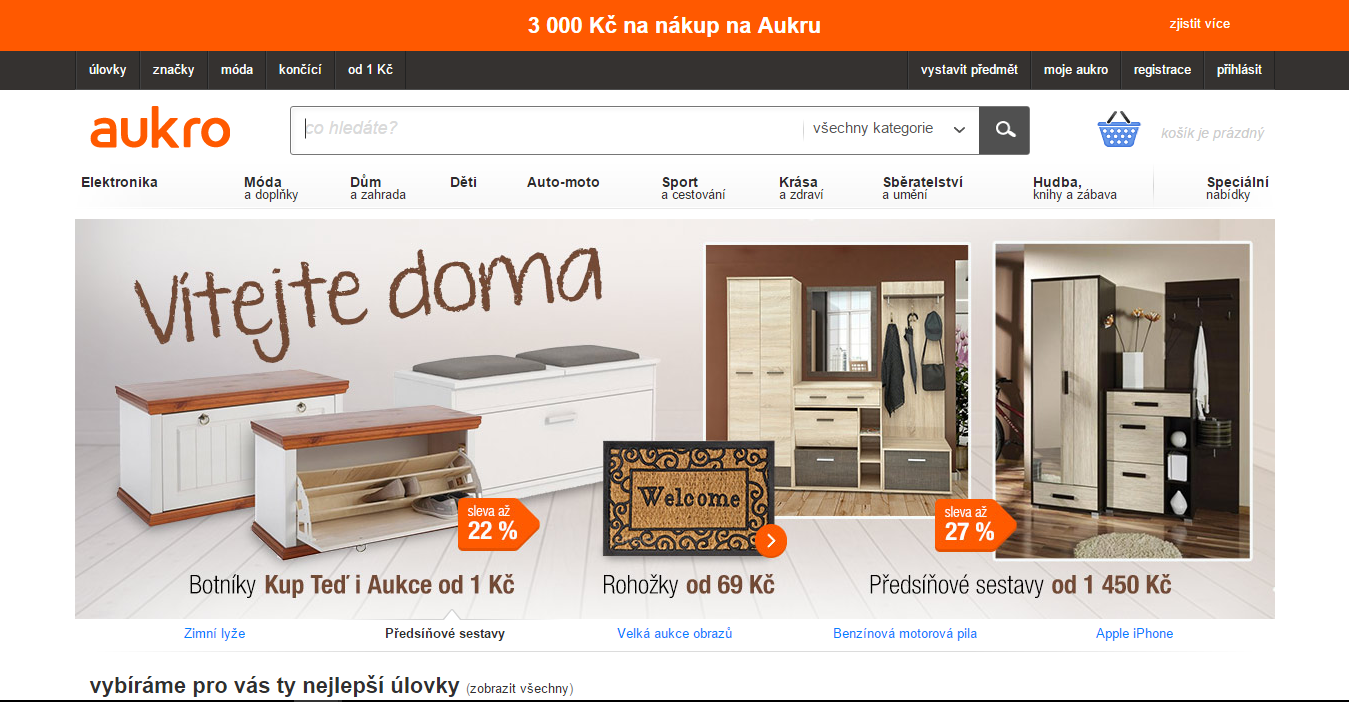
\includegraphics[width=1.0\textwidth]{media/aukro/home.png}
    \caption{Hlavní stránka webu Aukro.cz}
    \label{fig:aukro:home}
\end{figure}
\subsubsection*{Pozitiva}
\begin{itemize}
    \item[+] \textbf{Co hledáte?} -- Nejdůležitější prvek (vyhledávání) úvodní stránky je dostatečně velký a je na místě, kde ho uživatelé očekávají.
    \item[+] \textbf{Kategorie} -- Při najetí myší se kromě podkategorií zobrazí i populární kategorie a jedna speciální nabídka zboží. Myslím si, že toto chování způsobí, že si nějaká podskupina uživatelů nakoupí i něco, co předtím nechtěli, nebo to nebylo jejich prioritou.
\end{itemize}
\subsubsection*{Negativa}
\begin{itemize}
    \item[-] \textbf{Poutač} -- Velký poutač na speciální akce Aukra. Pokud chce uživatel vidět nějaké zboží, které mu vybralo aukro, nebo naposledy prohlédnuté zboží, tak musí přejít kolečkem myši poměrně dlouhý kus stránky.
\end{itemize}


%%%%%%%%%%%%%%%%%%%%%%%%%%%%%%%%%%%%%%%%%%%%%%%%%%%%%%%%%%%%%%%%%%%%%%%%%%%%%%%%%%%%%%%%%%%%%%%%%%%%%%%%%%%%%%%%%%%%%%%%

\newpage
\subsection{Vyhledávání zboží}
\begin{figure}[h]
    \centering
    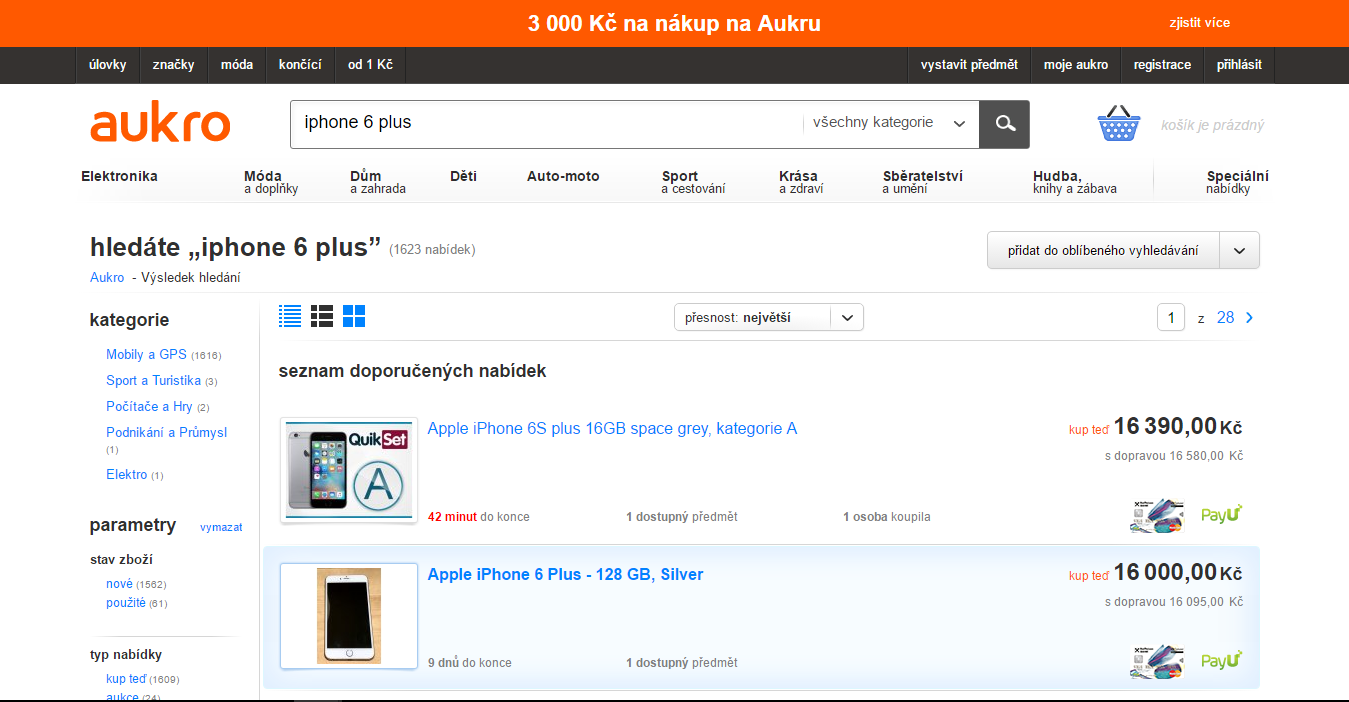
\includegraphics[width=1.0\textwidth]{media/aukro/search.png}
    \caption{Vyhledávání zboží na webu Aukro.cz}
    \label{fig:aukro:search}
\end{figure}
\subsubsection*{Pozitiva}
\begin{itemize}
    \item[+] \textbf{Cena i s dopravou} -- Na stránce je přímo zobrazená cena i s dopravou. Uživatel cítí určitou transparentnost a nemusí si tyto informace vyhledávat sám.
\end{itemize}
\subsubsection*{Negativa}
\begin{itemize}
    \item[-] \textbf{Málo informací o zboží} -- O konkrétním zboží se člověk kromě názvu moc nedozví. Místo na alespoň pár detailů tam přitom existuje.
    \item[-] \textbf{Málo nabídek} -- Dvě nabídky zaberou celou stránku ve výchozím nastavení.
    \item[-] \textbf{Chaotické rozhraní} -- Rozhraní je chaotické a neuspořádané.
\end{itemize}


%%%%%%%%%%%%%%%%%%%%%%%%%%%%%%%%%%%%%%%%%%%%%%%%%%%%%%%%%%%%%%%%%%%%%%%%%%%%%%%%%%%%%%%%%%%%%%%%%%%%%%%%%%%%%%%%%%%%%%%%

\newpage
\subsection{Detail zboží}
\begin{figure}[h]
    \centering
    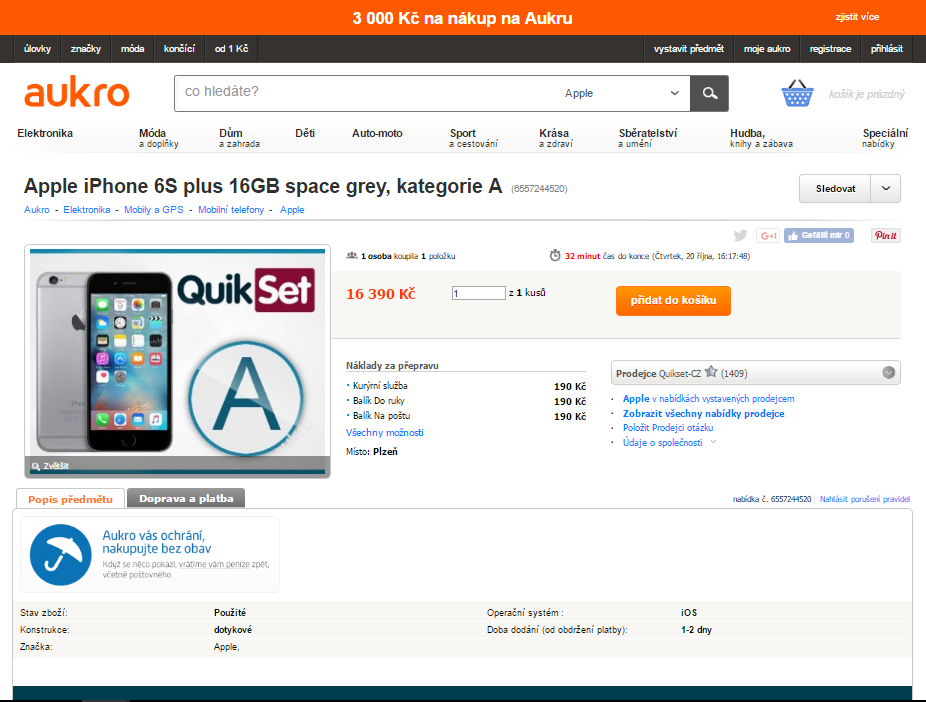
\includegraphics[width=1.0\textwidth]{media/aukro/detail.png}
    \caption{Detail zboží na webu Aukro.cz}
    \label{fig:aukro:detail}
\end{figure}
\subsubsection*{Pozitiva}
\begin{itemize}
    \item[+] \textbf{Nevidím}
\end{itemize}
\subsubsection*{Negativa}
\begin{itemize}
    \item[-] \textbf{Neobsahuje moc detailů} -- Detaily se nacházejí až ve spodní části stránky.
    \item[-] \textbf{Hodnocení prodejců} -- Sice se hodnocení prodejců na stránce nachází, ale výrazně je viditelnější až po rozkliknutí.
    \item[-] \textbf{Chaotické rozhraní} -- Problém uživatelského rozhraní zůstává.
\end{itemize}


%%%%%%%%%%%%%%%%%%%%%%%%%%%%%%%%%%%%%%%%%%%%%%%%%%%%%%%%%%%%%%%%%%%%%%%%%%%%%%%%%%%%%%%%%%%%%%%%%%%%%%%%%%%%%%%%%%%%%%%%

\newpage
\subsection{Profil prodejce}
\begin{figure}[h]
    \centering
    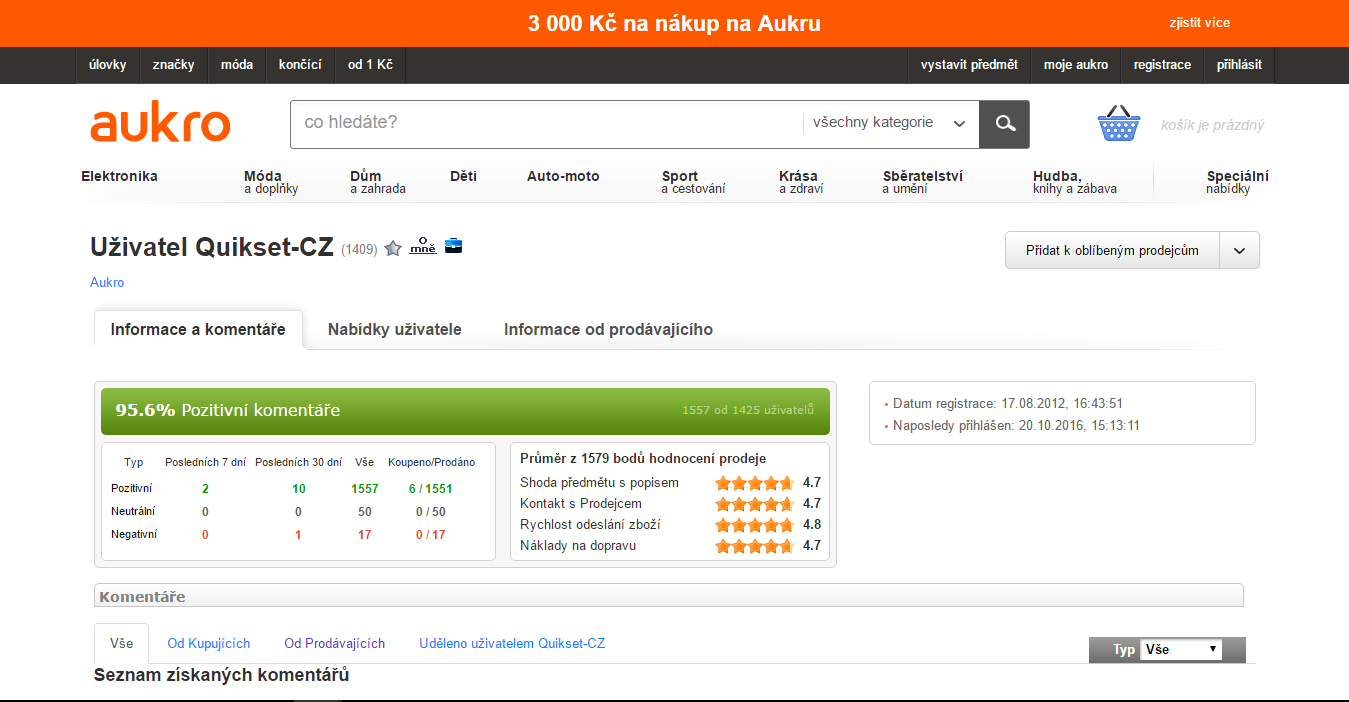
\includegraphics[width=1.0\textwidth]{media/aukro/profile.png}
    \caption{Profil prodejce na webu Aukro.cz}
    \label{fig:aukro:profile}
\end{figure}
\begin{figure}[h]
    \centering
    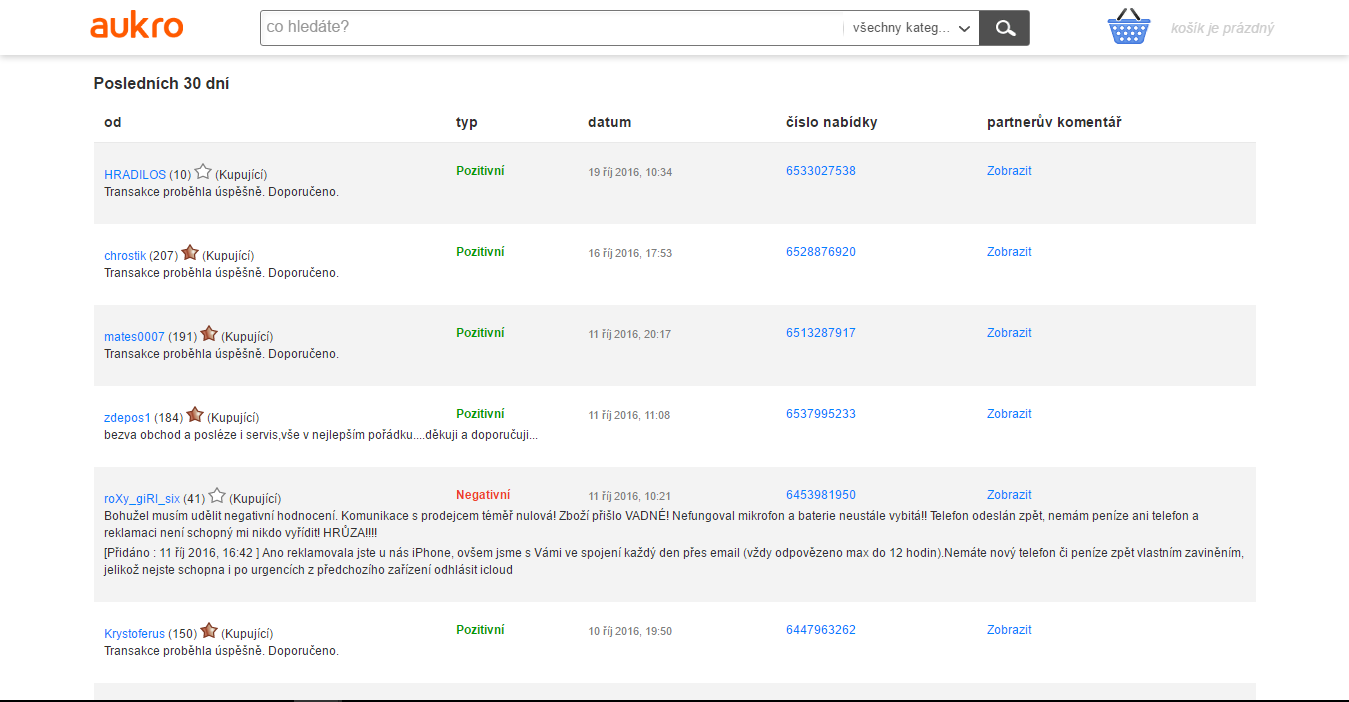
\includegraphics[width=1.0\textwidth]{media/aukro/profile2.png}
    \caption{Recenze uživatele na webu Aukro.cz}
    \label{fig:aukro:profile2}
\end{figure}
\subsubsection*{Pozitiva}
\begin{itemize}
    \item[+] \textbf{Historie hodnocení/komentářů} -- Možnost přečíst si kdo byl jak spokojený s daným prodejcem.
\end{itemize}
\subsubsection*{Negativa}
\begin{itemize}
    \item[-] \textbf{Nepřehlednost} -- Problémy s rozhraním se projevují i na této stránce. Nedá se vytvořit si závěry bez dlouhého kroucení kolečkem myši.
\end{itemize}


%%%%%%%%%%%%%%%%%%%%%%%%%%%%%%%%%%%%%%%%%%%%%%%%%%%%%%%%%%%%%%%%%%%%%%%%%%%%%%%%%%%%%%%%%%%%%%%%%%%%%%%%%%%%%%%%%%%%%%%%

\newpage
\subsection{Shrnutí}
Upřímně řečeno jsem při rešeršování Aukro.cz nabudil pocit, že chci z dané webové aplikace co nejdříve odejít. Z mých očekávání se nesplnilo nic a tak se musím poučit z chyb, kterých se dopustili. Konkrétně je to:
\begin{itemize}
    \item \textbf{Chaotické rozhraní}
    \item \textbf{Nedetailnost}
    \item \textbf{Málo poskytnutých informací}
\end{itemize}

Z mého pohledu se jeví být zajímavou funkcí \textbf{historie komentářů}, kdy si uživatel může vytvořit názor o prodejci . Chci však, aby mé rozhraní bylo přehledné a určitě aby poskytovalo všechny potřebné detaily. To pro mě znamená: jaká je daná nabídka, jak daleko je vzdálená a jaké hodnocení má prodejce - a to vše na jednom místě.
\newpage
\section{Zonky}
\label{chap:zonky}

Přímé půjčky od lidí, kteří rádi pomohou. Jinak řečeno - buďme lidští a vynechejme z toho banky. Princip, kterého se držím i v mé aplikaci.

\subsection{Home page}
\begin{figure}[h]
    \centering
    
\includegraphics[width=1.0\textwidth]{media/zonky/home.png}
    \caption{Hlavní stránka webu zonky.cz}
    \label{fig:zonky:home}
\end{figure}
\subsubsection*{Pozitiva}
\begin{itemize}
    \item[+] \textbf{Jednoduchost a přehlednost} -- Existence pouze pár tlačítek a jasná čitelnost všeho, co se na dané stránce nachází.
\end{itemize}
\subsubsection*{Negativa}
\begin{itemize}
    \item[-] \textbf{Zvuk} -- Velmi rušivý moment, který se zvýší v momentě když máte puštěnou na svém zařízení hudbu.
\end{itemize}


%%%%%%%%%%%%%%%%%%%%%%%%%%%%%%%%%%%%%%%%%%%%%%%%%%%%%%%%%%%%%%%%%%%%%%%%%%%%%%%%%%%%%%%%%%%%%%%%%%%%%%%%%%%%%%%%%%%%%%%%

\newpage
\subsection{Zlevnovač}
\begin{figure}[h]
    \centering
    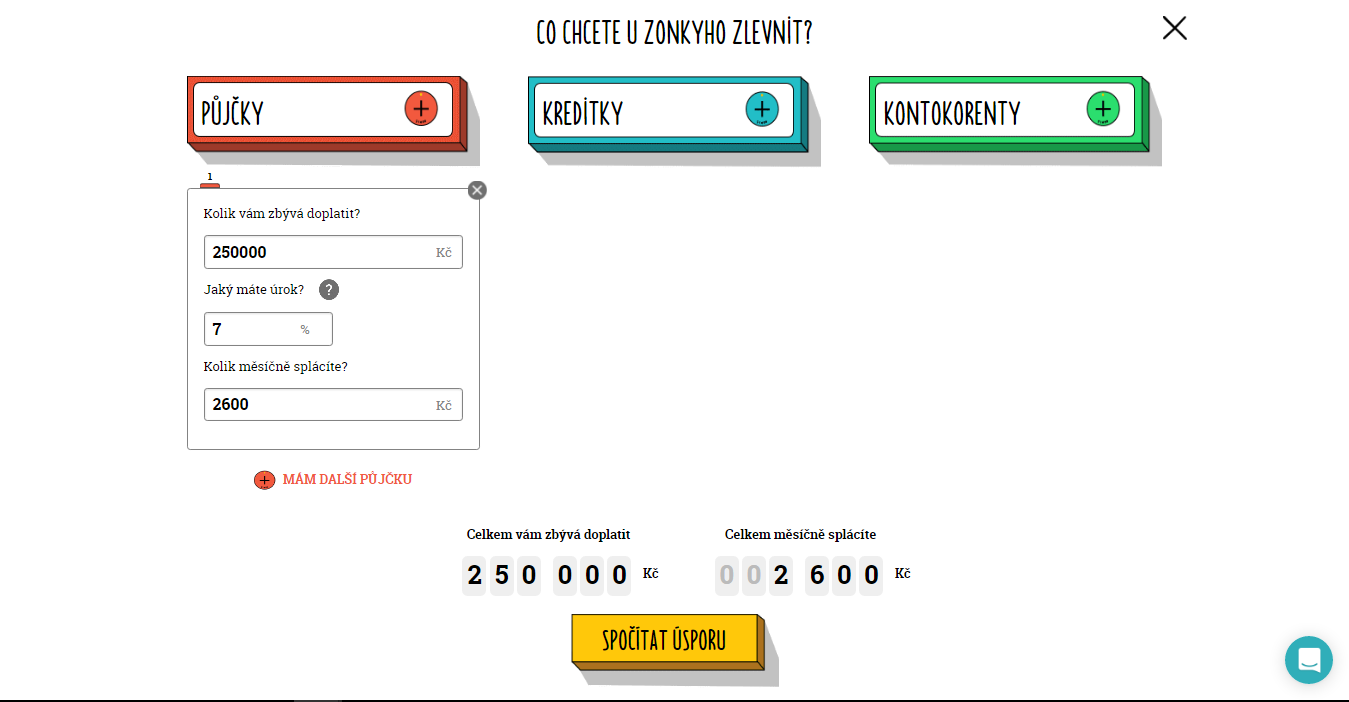
\includegraphics[width=1.0\textwidth]{media/zonky/zlevnovac.png}
    \caption{Zleňovač na webu zonky.cz}
    \label{fig:zonky:zlevnovac}
\end{figure}
\begin{figure}[h]
    \centering
    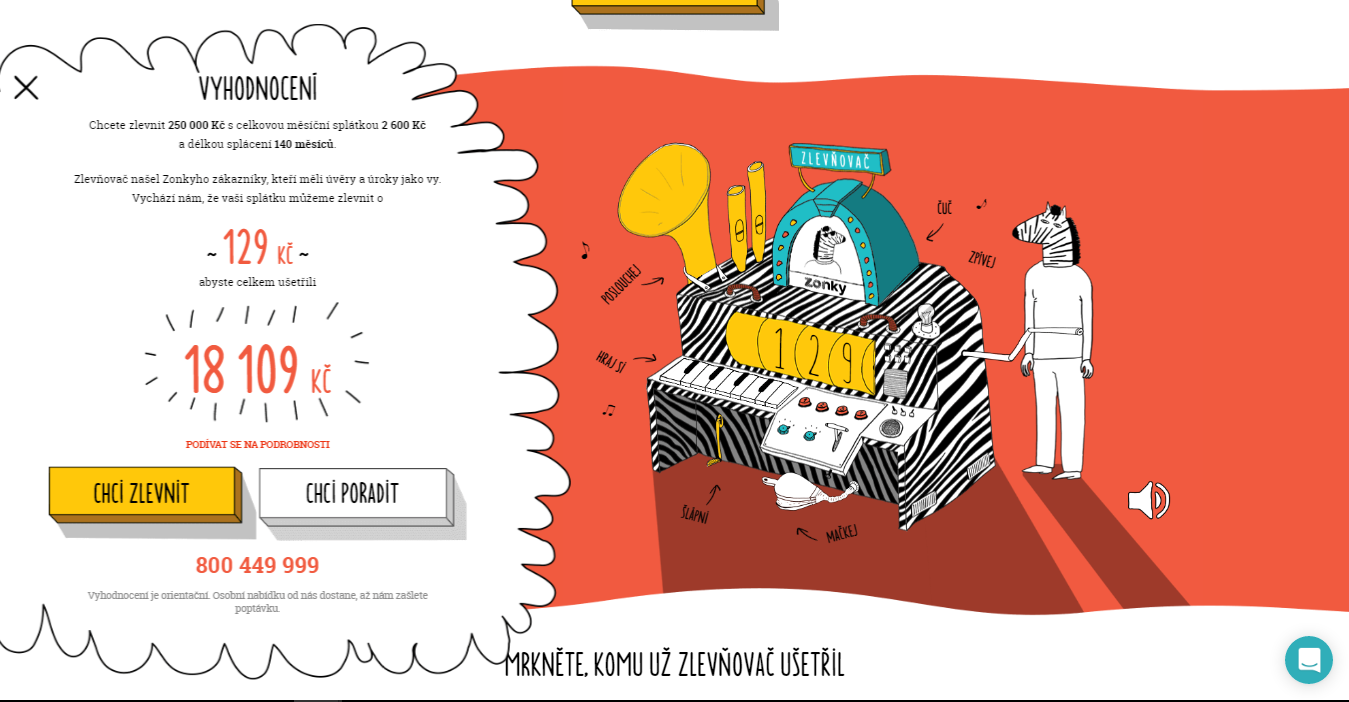
\includegraphics[width=1.0\textwidth]{media/zonky/zlevnovac2.png}
    \caption{Zlevňovač na webu zonky.cz 2}
    \label{fig:zonky:zlevnovac2}
\end{figure}
\subsubsection*{Pozitiva}
\begin{itemize}
    \item[+] \textbf{Jednoduchost a přehlednost} -- Opět jednoduché uživatelské rozhraní, ve kterém se nachází jen to potřebné.
    \item[+] \textbf{Vyhodnocení} -- Rychlý náhled na to kolik vlastně ušetřím, podaný pěknou a jasnou formou.
\end{itemize}
\subsubsection*{Negativa}
\begin{itemize}
    \item[-] \textbf{Zvuk}
\end{itemize}


%%%%%%%%%%%%%%%%%%%%%%%%%%%%%%%%%%%%%%%%%%%%%%%%%%%%%%%%%%%%%%%%%%%%%%%%%%%%%%%%%%%%%%%%%%%%%%%%%%%%%%%%%%%%%%%%%%%%%%%%

\newpage
\subsection{Tržiště}
\begin{figure}[h]
    \centering
    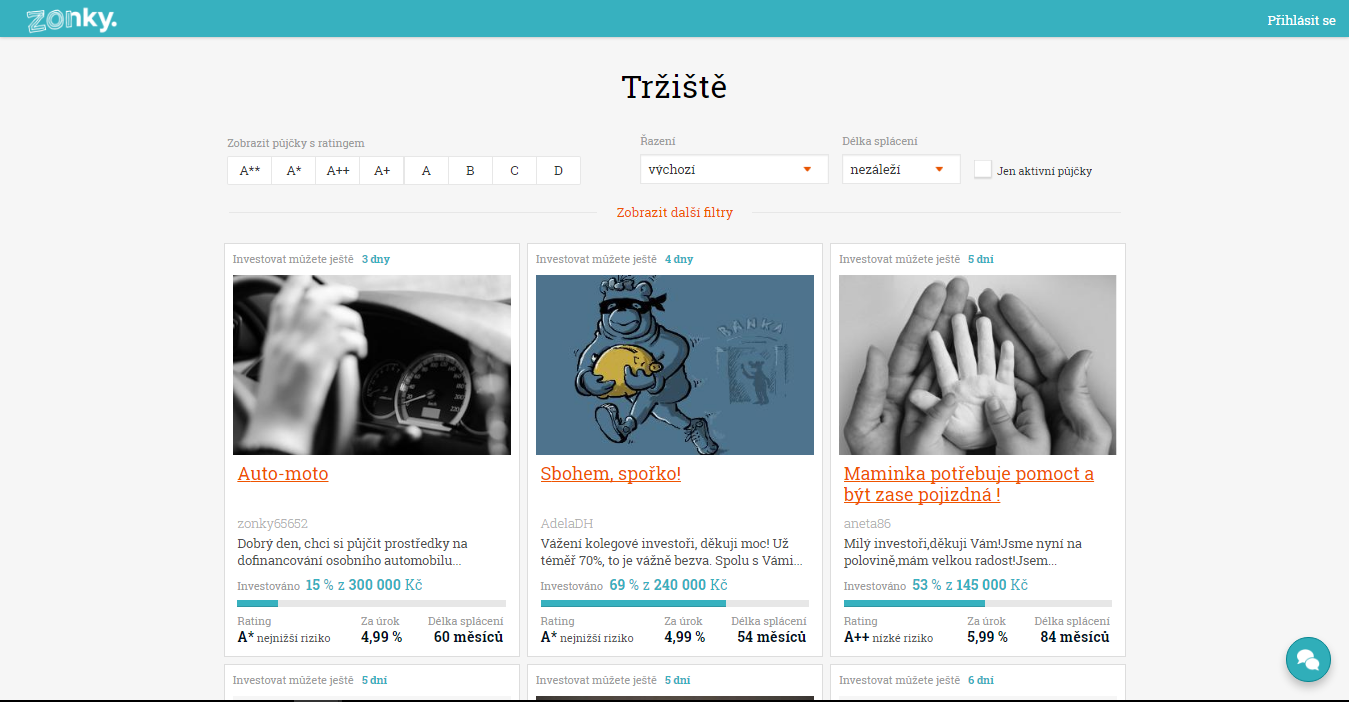
\includegraphics[width=1.0\textwidth]{media/zonky/marketplace.png}
    \caption{Tržiště na webu zonky.cz}
    \label{fig:zonky:marketplace}
\end{figure}
\subsubsection*{Pozitiva}
\begin{itemize}
    \item[+] \textbf{Informativnost} -- Krátký popis, rating, úrok a doba splácení je vše co uživatel na první pohled potřebuje.
    \item[+] \textbf{Filtry a řazení} -- Uživatel má šanci si rychle zobrazit nabídky, které ho zajímají.
\end{itemize}
\subsubsection*{Negativa}
\begin{itemize}
    \item[-] \textbf{Nevidím}
\end{itemize}


%%%%%%%%%%%%%%%%%%%%%%%%%%%%%%%%%%%%%%%%%%%%%%%%%%%%%%%%%%%%%%%%%%%%%%%%%%%%%%%%%%%%%%%%%%%%%%%%%%%%%%%%%%%%%%%%%%%%%%%%

\newpage
\subsection{Návodné a informatívní stránky}
\begin{figure}[h]
    \centering
    
\includegraphics[width=1.0\textwidth]{media/zonky/info.png}
    \caption{Když lidé půjčují lidem -- zonky.cz}
    \label{fig:zonky:info}
\end{figure}
\begin{figure}[h]
    \centering
    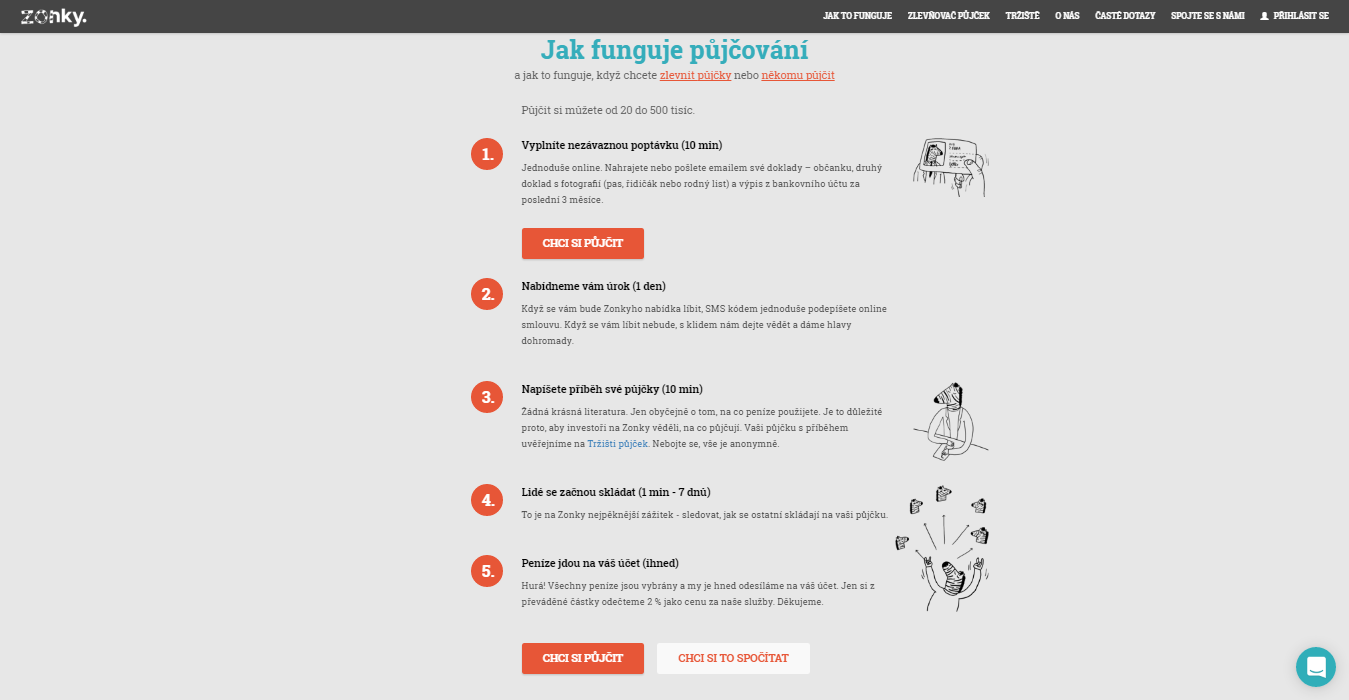
\includegraphics[width=1.0\textwidth]{media/zonky/info2.png}
    \caption{Jak funguje půjčování -- zonky.cz}
    \label{fig:zonky:info2}
\end{figure}
\begin{figure}[h]
    \centering
    
\includegraphics[width=1.0\textwidth]{media/zonky/info3.png}
    \caption{O lidech -- zonky.cz}
    \label{fig:zonky:info3}
\end{figure}
\subsubsection*{Pozitiva}
\begin{itemize}
    \item[+] \textbf{Uživatelská přívětivost} -- Informace podané snadně, jednoduše a přehledně skrz naskrz. Nic není zbytečně rozsáhlé.
\end{itemize}
\subsubsection*{Negativa}
\begin{itemize}
    \item[-] \textbf{Nevidím}
\end{itemize}


%%%%%%%%%%%%%%%%%%%%%%%%%%%%%%%%%%%%%%%%%%%%%%%%%%%%%%%%%%%%%%%%%%%%%%%%%%%%%%%%%%%%%%%%%%%%%%%%%%%%%%%%%%%%%%%%%%%%%%%%

\newpage
\subsection{Shrnutí}
Zonky.cz deklaruje, že chce pomoci lidem, resp. poskytuje možnost pro lidi pomáhat si navzájem. Já chci od své webove aplikace stejnou věc a proto bych se mohl z tohoto řešení něco přiučit.

Pokud chci pomáhat lidem, tak mé uživatelské rozhraní musí být příjemné na používání (to znamená \textbf{jednoduché a přehledné}). Určite se toho dá dosáhnout i zvolením jiného typu grafiky, ale myšlenka zůstává. Dále si všímám, že v každém zákoutí Zonky se k nám dostává \textbf{ dostatečné množství informací} (nejsme zahlcení) a tento princip implementuji také. \textbf{Přítomnost zvuku} je velmi odrazující a určitě tuto chybu nezopakuji v mé aplikaci.
